%
% File eamt20.tex
%
% Contact: cettolo@fbk.eu, mlf@dlsi.ua.es

%%% To ease future customizations, various replaceables have been paramaterized
%%% as listed in the newcommands section

\documentclass[11pt]{article}
\usepackage{eamt22}
\usepackage{times}
\usepackage{url}
\usepackage{latexsym}
\usepackage[small,bf]{caption} % added MLF 20171211
\setlength\titlebox{6.8cm}    % Expanding the titlebox
%%% YOUR PACKAGES BELOW THIS LINE %%%

\newcommand{\confname}{EAMT 2022}
\newcommand{\website}{https://eamt2022.com/}
\newcommand{\urlwebsite}{https://eamt2022.com/}
\newcommand{\contactname}{the guest organizers, LT3,}
\newcommand{\contactemail}{\texttt{eamt2022@ugent.be}}
\newcommand{\conffilename}{eamt22}
\newcommand{\downloadsite}{https://eamt2022.com/templates}

\newcommand{\paperlength}{$10$ (ten)}
\newcommand{\shortpaperlength}{$10$ (ten)}
\newcommand{\projectlength}{$2$ (two)}
\newcommand{\translatorlength}{$10$ (ten)}

\title{Multi-Domain Adaptation in Neural Machine Translation with Dynamic Sampling Strategies}

%\author{First Author\\
%  Affiliation / Address line 1\\
%  Affiliation / Address line 2\\
%%  Affiliation / Address line 3\\
%  {\tt email@domain}  \And
%  Second Author\\
%  Affiliation / Address line 1\\
%  Affiliation / Address line 2\\
%%  Affiliation / Address line 3\\
%  {\tt email@domain}}

\author{Minh-Quang Pham\\
  Uni. Paris-Saclay,  CNRS, LISN \\
  F-91405 Orsay \\
  {\tt pham@limsi.fr}  \And
  Josep Crego\\
  SYSTRAN ,\\
  5 rue Feydeau, F-75002 Paris\\
  {\tt crego@systrangroup.com} \And
  Fran\c cois Yvon\\
  Uni. Paris-Saclay, CNRS, LISN\\
  F-91405 Orsay, France\\
  {\tt yvon@limsi.fr}}

\date{}
% This assumes your files are encoded as UTF8
\usepackage[utf8]{inputenc}
\renewcommand{\UrlFont}{\ttfamily\small}
\usepackage{graphicx}
\usepackage{grffile}
\usepackage{multirow}
\usepackage{xcolor,colortbl}
\usepackage{amsmath}
%\usepackage{fdsymbol}
\usepackage{amssymb}
\usepackage{makecell}
\usepackage[super]{nth}
\usepackage{arydshln}
\usepackage{algorithm,algorithmic}

%\usepackage[noend]{algpseudocode}
% \usepackage{regexpatch}
% \usepackage{subcaption}
% This is not strictly necessary, and may be commented out,
% but it will improve the layout of the manuscript,
% and will typically save some space.
\usepackage{microtype}

\usepackage{longtable}
\usepackage{tikz}
\usetikzlibrary{calc}
\usepackage[draft]{todo}
\usepackage[normalem]{ulem}
\usepackage{xspace}
\usepackage{float}

\usepackage{pgfplots}
\usepackage{pgfplotstable}

%\let\oldbibitem\bibitem
% \def\bibitem{\vfill\oldbibitem}

\usepackage{soulutf8}
\usepackage{tabularx}
\usepackage{adjustbox}
\usepackage{subcaption}
% \usepackage{hyperref}

\newcommand{\fyTodo}[1]{\Todo[FY:]{\textcolor{orange}{#1}}}
\newcommand{\fyTodostar}[1]{\Todo*[FY:]{\textcolor{orange}{#1}}}
\newcommand{\fyDone}[1]{\done[FY]\Todo[FY:]{\textcolor{orange}{#1}}}
\newcommand{\fyFuture}[1]{\done[FY]\Todo[FY:]{\textcolor{red}{#1}}}
\newcommand{\fyDonestar}[1]{\done[FY]\Todo[FY:]{\textcolor{orange}{#1}}}

\newcommand{\revision}[1]{\textcolor{red}{#1}}
\newcommand{\revisiondel}[1]{}
\newcommand{\src}{\ensuremath{\mathbf{f}}} % source sentence
\newcommand{\trg}{\ensuremath{\mathbf{e}}} % target sentence
\newcommand{\domain}[1]{\texttt{\textsc{#1}}}
\newcommand{\system}[1]{\texttt{{#1}}}

\newcommand{\vlambda}{\ensuremath{\boldsymbol\lambda}\xspace} % parameters vector for a distribution
\newcommand{\vtheta}{\ensuremath{\boldsymbol\theta}\xspace} % parameters vector for a distribution
\newcommand{\vpsi}{\ensuremath{\boldsymbol\psi}\xspace} % parameters vector for a distribution
\newcommand{\indic}[1]{\ensuremath{\mathbb{I}(#1)}}
% \newcommand{\SB}[1]{\textcolor{green}{#1}}
% \newcommand{\SW}[1]{\textcolor{red}{#1}}
\newcommand{\SB}[1]{\textbf{#1}}
\newcommand{\SW}[1]{\underline{#1}}
% limits underneath
\DeclareMathOperator*{\argmin}{arg\,min}
\DeclareMathOperator*{\argmax}{arg\,max}
\renewcommand\textfraction{.1}
\renewcommand\floatpagefraction{.95}
\newcommand{\sbcl}[2]{{\scriptsize #1 \hfill $|$ \hfill  #2}}

\makeatletter
\newenvironment{breakablealgorithm}
  {% \begin{breakablealgorithm}
   \begin{center}
     \refstepcounter{algorithm}% New algorithm
     \hrule height.8pt depth0pt \kern2pt% \@fs@pre for \@fs@ruled
     \renewcommand{\caption}[2][\relax]{% Make a new \caption
       {\raggedright\textbf{\fname@algorithm~\thealgorithm} ##2\par}%
       \ifx\relax##1\relax % #1 is \relax
         \addcontentsline{loa}{algorithm}{\protect\numberline{\thealgorithm}##2}%
       \else % #1 is not \relax
         \addcontentsline{loa}{algorithm}{\protect\numberline{\thealgorithm}##1}%
       \fi
       \kern2pt\hrule\kern2pt
     }
  }{% \end{breakablealgorithm}
     \kern2pt\hrule\relax% \@fs@post for \@fs@ruled
   \end{center}
  }
\makeatother

\begin{document}
\maketitle
\setlength{\abovedisplayskip}{2pt}
\setlength{\belowdisplayskip}{2pt}
\begin{abstract}
  Building effective Neural Machine Translation models often implies accommodating diverse sets of heterogeneous data so as to optimize performance for the domain(s) of interest. Such multi-source / multi-domain adaptation problems are typically approached through instance selection or reweighting strategies, based on a static assessment of the relevance of training instances with respect to the task at hand. In this paper, we study dynamic data selection strategies that are able to automatically re-evaluate the usefulness of data samples
  % and to evolve a data selection policy
  in the course of training. Based on the results of multiple experiments, we show that our method offer a generic framework to automatically
  % and effectively
  handle several real-world situations, from multi-source or unsupervised domain adaptation to multidomain learning.
\end{abstract}

\section{Introduction}\label{sec:intro}
A typical setting in machine translation (MT) is to collect the largest possible collection of parallel data for the chosen language pair, with the intent to achieve optimal performance for the task of interest. In such situations, the training data distribution is opportunistic, while the test data distribution is chosen and fixed; a key aspect of training is then to mitigate the detrimental effects of a mismatch between these distributions. Single-source and multi-source\footnote{In this paper, multi-source DA means having multiple domains to adapt from; this setting differs from multi-source translation, where several \emph{source languages} are considered.} domain adaptation (DA) is a well-studied instance of this setting (see \cite{Chu2017comparison,Saunders21asurvey} for a review), and so is multi-domain (MD) learning \cite{Chu18multilingual,Zeng18multidomain,Jiang19multidomain,Pham21revisiting}. A related situation is multilingual MT \cite{Firat16multiway,Ha16towards,Johnson17google,Aharoni19massively},\fyDone{Fix ref}
% \revision{cite also \cite{Shen21source}} -> I think this is not so appropriate here
where the diversity of training data not only corresponds to variations in the topic, genre, or register but also in language.

This problem is often approached by \emph{static} instance selection or re-weighting strategies, where the available training data is used in proportion to its relevance for the testing conditions \cite{Moore10selection,Axelrod11domain}. Finding the optimal balance of training data is however, a challenging task due, for instance, to the similarity between domains/languages, or to the regularization effects of out-of-domain data \cite{Miceli-barone17regularization}. A static policy may also be suboptimal when some target domains or languages are easier to train than others. Finally, improving the performance of the MT system in one domain will often hurt that of another \cite{Vanderwees17dynamic,Britz17mixing} and improving model generalization across all domains \cite{koehn18findings} may not achieve optimally for any particular domain. 

Several recent proposals
% \cite{Vanderwees17dynamic,Graves17automated,platanios19competence,Zhang19curriculum,Kumar19reinforcement,Wang20learning-multi,Wang20balancing,Wang20learning-multi}
explore ways to instead consider \emph{dynamic} data selection and sampling strategies: \newcite{Vanderwees17dynamic} and \newcite{Zhang19curriculum} construct a static curriculum, while \newcite{Wang20learning-multi} and \newcite{Wang20balancing} build curricula that automatically adapt to the training data. In this paper, we contribute to this line of research in several ways. 
\begin{itemize}
	\item First, we propose a novel framework (\emph{Multi-Domain Automated Curriculum}, MDAC for short), a variant of Differentiable Data Selection (DDS) of \newcite{Wang20balancing}, initially applied to multilingual NMT, that simultaneously accounts for the domain adaptation and the multidomain adaptation problems.
	\item We show that MDAC achieves performance that compare to fine-tuning strategies for DA (\textsection~\ref{ssec:da}) and outperform some static data sampling strategies for multidomain settings (\ref{ssec:mda}).
	\item We show that our variant MDAC mitigates some failures of DDS in multidomain training.
	\item We illustrate the generality of differentiable data selection frameworks (both MDAC and DDS) on less common situations such as DA using unsupervised clustering (\textsection~\ref{ssec:clda}); DA using out-of-domain training data and small in-domain validation data (\textsection~\ref{ssec:uda}); and two-domain adaptation where the test distribution only mixes two of the training domain (\textsection~\ref{ssec:bida}).
\end{itemize}


\section{Learning with multiple data sources} \label{sec:mdmt}

We conventionally define a domain $d$ as a distribution $\mathcal{D}_d(x)$ over some feature space $\mathcal{X}$ that is shared across domains \cite{Pan10asurvey}: in machine translation, $\mathcal{X}$ is the representation space for input sentences; each domain corresponds to a specific source of data, and may differ from other data sources in terms of textual genre, thematic content \cite{Chen16guided,Zhang16topicinformed}, register, style \cite{Niu18multitask}, etc. Translation in domain $d$ is formalized by a translation function $h_d(y|x)$ pairing sentences in a source language with sentences in a target language $y \in \mathcal{Y}$. $h_d$ is usually assumed to be deterministic (hence $y = h_d(x)$) but may differ across domains.

It is usual in MT to opportunistically collect corpora from several domains, which means that training instances are distributed according to a mixture $\mathcal{D}^s$ such that $\mathcal{D}^s(x) = \sum_{d=1}^{n_d} \lambda^{s}(d) \mathcal{D}_d(x)$, with $\{\lambda^{s}(d), d=1 \dots n_d\}$ the mixture weights satisfying $\sum_d \lambda^{s}(d)=1$. In the sequel, boldface $\vlambda$ denotes a vector with $\lambda(d)$ the $d^{th}$ component of $\vlambda$.

The main challenge in this situation is to make the best of heterogeneous data, with the aim to achieve optimal performance for the target test conditions. These might correspond to data from just one of the training domains, as in standard supervised domain adaptation; a more difficult case is when the test data is from one domain unseen in training (unseen domain adaptation); in multidomain adaptation finally, the test distribution is itself a mixture of domains, some of which may also be observed in training. We thus assume that the test distribution takes the form $\mathcal{D}^{t}(x) = \sum_d \lambda^{t}(d) \mathcal{D}_d(x)$ - with only one non-null  component in the case of domain adaptation (see Figure~\ref{fig:mdmt-lambdas}).
\begin{figure}[h]
  \centering
  \vspace{-\baselineskip}
  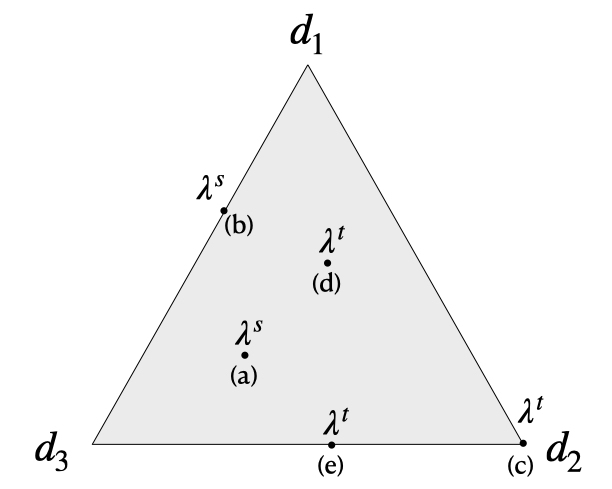
\includegraphics[width=0.48\textwidth]{mdmt-lambdas}
  \caption{Training and testing with distribution mismatch. We consider three domains and represent $\vlambda^{s}$ and $\vlambda^{t}$ in the 3-dimensional simplex. Training with weights in (a) and testing with weights in (c) is supervised multi-source domain adaptation to domain~2 ($d_2$), while (b)-(c) is the unsupervised version, with no training data from $d_2$; training with weights in (a) and testing with weights in (d) is multi-domain learning, also illustrated with settings (a)-(e) (training domain $d_1$ is not seen in test), and (b)-(d)  (test domain $d_2$ is unseen in training).}\label{fig:mdmt-lambdas}
\end{figure}

These situations have been amply documented from a theoretical perspective \cite{Mansour09multiple,Mansour09domainadaptation,Hoffman18algorithms}. A general recommendation in the DA setting is to adjust the sampling distribution used to optimize the system so as to compensate for the mismatch between $\mathcal{D}^s(x)$ and $\mathcal{D}^t(x)$. This can be approximated by reweighting instances, or more conveniently domains, which are selected during training with a probability $\lambda^{l}(d)$, with $\lambda^{l}(d) \neq \lambda^{s}(d)$.

A widely-used approach to supervised DA is \emph{fine-tuning} \cite{Luong15stanford}, where $\vlambda^{l}$ varies during learning. With our notations, this approach first learns an initial parameter value with all the data ($\forall d, \lambda^{l}(d) = \lambda^{s}(d)$), then continues training with only batches from the test domain $d_t$ ($\lambda^{l}(d) = \indic{d = d_t}$), with $\indic{A}$ the indicator function for predicate $A$. This strategy is potentially suboptimal as some out-of-domain samples may contribute to the final performance due to e.g.\ domain similarity. Optimizing the learning distribution in multidomain settings is even more challenging as the learner needs to take advantage of possible domains overlaps and also of the fact that some domains might be easier to learn than others.\fyDone{How to measure this?}
% \revision{Answer: The graphic of \system{Mixed-0} shows that with the same amount of data(batches) the convergences of the domains vary significantly}

\section{Multi-Domain Automated Curriculum } \label{sec:mdac}
\subsection{Basic principles}
Assuming training data in each of the $n_d$ domains $d_1 \dots d_{n_d}$, the size of the training corpus in domain $d$ is denoted $N^{s}_d$, and $N^{s} = \sum_d N^{s}_d$ is the total number of training samples. $\widehat{\mathcal{D}^l_d}$ and $\widehat{\mathcal{D}^t_d}$ denote the empirical train and test distributions for domain $d$ and $\widehat{\mathcal{D}^{u}}(x;\vlambda^{u}) = \sum_{d} \lambda^{u}(d) \widehat{\mathcal{D}^{u}_d}(x)$ for $u\in\{l,t\}$. In our setting,  $\vlambda^{t}$ and hence $\widehat{\mathcal{D}^t}(x;\vlambda^t)$ are fixed and predefined, approximated with an equivalent number of development corpora. 

% Our method
MDAC builds an adaptative training distribution $\vlambda^{l}$ that optimizes the data selection policy along with the training of the model. We parameterize $\vlambda^{l}$ by a differentiable function $\vlambda^l(\psi)$, which is described in \textsection~\ref{ssec:dds-sys}. We divide the training into many short sessions; in each session $t$, the model is trained with a static data distribution $\vlambda^{l}(\psi_t)$. After one learning session, we update the data distribution using the REINFORCE algorithm of \newcite{Williams92simple}. The evolution of $\psi$ is thus defined by:\fyDone{$t$ is both for time, and for test - change into $\tau$?}
\begin{align*}
\psi_{t+1} &= \psi_t + \mathbf{lr}_{1} * \displaystyle{\mathop{\sum}_{d=1}^{n_d}} R(d) * \frac{\partial \lambda^l(d;\psi_t)}{\partial \psi},
\end{align*}
\begingroup
\allowdisplaybreaks
where the reward $R(d)$ is computed as:
\begin{align}
  R(d) = J^t(\theta_{t+k},\vlambda^t) - J^t(\theta_t,\vlambda^t), \label{eq:reward}
\end{align}
and where we also define:
\begin{equation}
\begin{array}{rcl}
\theta_{t+i} &=& Update\big(\theta_{t+i-1},[x^i_j,y^i_j]_{j=1}^N\big) \\ \nonumber
x^i_j, y^i_j &\sim& \widehat{D^l_d}(x) \\
J^t(\theta,\vlambda^t) &=& \displaystyle{\mathop{\sum}_{d=1}^{n_d}}\lambda^t(d)\displaystyle{\mathop{\sum}_{x^t_d,y^t_d \in \widehat{D^t_d}}} l(\theta,x^t_d,y^t_d).
\end{array}
\end{equation}
\endgroup
% \theta_{t+i-1} - \mathbf{lr_2} \frac{1}{N}\displaystyle{\mathop{\sum}_{j=1}^N}\frac{\partial l(\theta_{t+i-1}, x^i_j,y^i_j)}{\partial \theta}
In these equations, $N$ denotes the size of a batch; $\mathbf{lr}_{1}$ is the learning rate of the sampling distribution; $l(\theta,x,y)$ is the loss of the NMT model on sample $(x,y)$; $J^t(\theta,\vlambda^t)$ is the weighted loss aggregated over $n_d$ dev-sets corresponding to the $n_d$ domains.

To compute the reward $R(d)$ associated to training the model with data from domain $d$, we simulate $k$ training steps from the current checkpoint, using $k$ batches sampled from $D^l(d)$ and computing the gain of the weighted dev-loss. This computation is inspired by the target prediction gain of \newcite{Graves17automated}. However, where \newcite{Graves17automated} used accumulated gains from the past as rewards, we instead predict the usefulness of each domain for improving the future performance of the system given its current state. This is achieved by simulating a round of training with only the data from one domain. We also differ from these authors in the parameterization of the sampling distribution.
% Furthermore, the choice of the parameterization of the sampling distribution in our method differs from that of \newcite{Graves17automated}, although this choice is empirical.

The work of \newcite{Wang20balancing} is also related: it is based on the bi-level optimization framework, which aims to find an optimal static distribution $\vlambda^{l}$ that will result in the best model with respect to a given target dev set at the end of training. These authors also derive a similar form of update for $\psi$. However, their reward is the cosine similarity between the gradient computed with the training data from one domain and the gradient computed with the dev set. We compare this approach with ours in the experiment section.

\subsection{MDAC for (multi) domain adaptation}
The setting developed in previous sections is quite general and can, in principle, accommodate the variety of situations mentioned above, and many more: basic DA, multidomain adaptation with various target distributions, possibly including domains unseen in training. In our experiments, we would like to better assess the potential of MDAC in these settings and seek to study the following questions:
\begin{itemize}
\item is MDAC a viable alternative to fine-tuning? In particular, does it enable to better take advantage of relevant data from other domains?
\item is MDAC a viable option in multidomain adaptation scenarios?
\item does MDAC enable to perform \emph{unsupervised} (multi-)domain adaptation? \fyDone{TBContinued}
\end{itemize}
These questions are further explored in Section~\ref{sec:results}. We now turn to our experimental conditions.

\section{Experimental settings} \label{sec:exp}
\subsection{Data and metrics \label{ssec:corpora}}
\begin{table*}[htbp]
  \vspace{-\baselineskip}
  \centering \footnotesize
  \begin{tabular}{|l|ccccccc|} %*{4}{|r|}}
    \cline{2-8} 
    %\multicolumn{4}{|l|}{Vocab size - En: 30,165, Fr: 30,398}\\
    \multicolumn{1}{c|}{} & \multicolumn{1}{c}{\domain{med}} & \multicolumn{1}{c}{\domain{law}} & \multicolumn{1}{c}{\domain{bank}} & \multicolumn{1}{c}{\domain{it}} & \multicolumn{1}{c}{\domain{talk}} & \multicolumn{1}{c}{\domain{rel}} & \multicolumn{1}{c|}{\domain{news}} \\
    \hline 
    \# lines & 2609 (0.68) & 501 (0.13) & 190 (0.05) & 270 (0.07) & 160 (0.04) & 130 (0.03) & 260 (0) \\
    \# tokens &  133 / 154  &  17.1 / 19.6 &  6.3 / 7.3 &  3.6 / 4.6 &  3.6 / 4.0 &  3.2 / 3.4 & 7.8 / 9.2   \\
    \# types & 771 / 720 & 52.7 / 63.1 & 92.3 / 94.7 & 75.8 / 91.4 & 61.5 / 73.3 & 22.4 / 10.5 & - \\
    \# uniq & 700 / 640 & 20.2 / 23.7 & 42.9 / 40.1 & 44.7 / 55.7 & 20.7 / 25.6 & 7.1 / 2.1 & - \\
    \hline
  \end{tabular}
  \caption{Corpora statistics: number of parallel lines ($\times 10^3$) and proportion in the training domain mixture (exluding \domain{news}), number English and French tokens ($\times 10^6$), types and uniq types ($\times 10^3$): the latter are types that only appear in a given domain.
    % \domain{med} is the largest domain, containing almost 70\% of the sentences, while \domain{rel} is the smallest, with only 3\% of the data.
  }
  \vspace{-\baselineskip}
\label{tab:Corpora}
\end{table*}

We experiment with translation from English into French in 6~domains, corresponding to the following data sources: the UFAL Medical corpus V1.0 (\domain{med})\footnote{\url{https://ufal.mff.cuni.cz/ufal_medical_corpus}. We only use the in-domain (medical) subcorpora: PATR, EMEA, CESTA, ECDC.}; the European Central Bank corpus (\domain{bank}); the JRC-Acquis Communautaire corpus (\domain{law}) \cite{Steinberger06acquis}; documentations for KDE, Ubuntu, GNOME and PHP from the Opus collection, merged in a \domain{it}-domain; TedTalks (\domain{talk}) \cite{Cettolo12wit}, and the Koran (\domain{rel}). Additional experiments use the News Commentary corpus (\domain{news}). Most corpora are available from the Opus website\footnote{\url{http://opus.nlpl.eu}}. These corpora were deduplicated and tokenized with in-house tools; statistics are in Table~\ref{tab:Corpora}. To reduce the number of types, we use Byte-Pair Encoding \cite{Sennrich16BPE} with 30,000 merge operations on a corpus containing all sentences in both languages.\fyDone{Add \# number of tokens, also specificity ?}%
%
We randomly select in each corpus a development and a test set of 1,000 lines and keep the rest for training. Validation sets are used to chose the best model according to the average BLEU score \cite{Papineni02bleu}.\footnote{We use truecasing and \texttt{sacrebleu} \cite{Post18call}.}\fyDone{A word about meta-parameter settings} Significance testing is performed using bootstrap resampling \cite{Koehn04statistical}, implemented in compare-mt\footnote{\url{https://github.com/neulab/compare-mt}} \cite{Neubig19compare-mt}. We report significant differences at the level of $p=0.05$.\fyDone{Fix correct p value}

\subsection{Baseline systems \label{ssec:baseline}}
Our baselines are standard for multidomain settings.\footnote{We however omit domain-specific systems trained only with the corresponding subset of the data, which are always inferior to the mix-domain strategy \cite{Britz17mixing}.} Using Transformers \cite{Vaswani17attention} implemented in OpenNMT-tf\footnote{\url{https://github.com/OpenNMT/OpenNMT-tf}} \cite{Klein17opennmt}, we build the following systems:
\begin{itemize}
\itemsep0em 
\item Generic models trained with predefined mixtures of the training data taking the form:
\begin{align} \label{mixture:trn}
\lambda_{\alpha}(d) = (\sum_{d=1}^{n_d}q_d^{\alpha})^{-1} (q_d^{\alpha}) &&
q_d = \frac{\mid N^{s}_d \mid}{\displaystyle{N^{s}}} % \mathop{\sum}_{i=1}^K\mid D_i \mid}}
\end{align}
%\setlength{\abovedisplayskip}{2pt}
% \setlength{\belowdisplayskip}{2pt} 
with $\alpha \in \{0,0.25,0.5,0.75,1.0\}$. We denote these as \system{Mixed-$\alpha$} below. \system{Mixed-$0$} uses a uniform distribution, \system{Mixed-$1.0$} the empirical distribution of domains.
\item fine-tuned models based on \system{Mixed-$1.0$}, further trained on each domain for at most 50~000 iterations, with early stopping when the dev BLEU stops increasing for 5 successive iterations.\fyDone{for ?? iterations} The fine-tuning (\system{FT-Full}) procedure updates all the parameters of the initial model, resulting in six systems, one per domain, with no parameter sharing across domains.
\item systems trained with fixed mixtures with $\vlambda^l \in \big[ \vlambda_0, \vlambda_{0.25}, \vlambda_{0.5}, \vlambda_{0.75}, \vlambda_{1.0}\big]$; these are used in the multidomain experiments of \textsection~\ref{ssec:mda};
\item  our implementations of dynamic sampling proposals from the literature: Curriculum Learning (CL) of \newcite{Zhang19curriculum} and Differential Data Selection (DDS) of \newcite{Wang20balancing} (see below);
\end{itemize}

All models use embeddings and hidden layers of dimension~512. Transformer models contain 8~attention heads in each of the 6+6 layers; the inner feedforward layer contains 2048 cells. Training lasts for 200K iterations, with batches of~12,288 tokens, Adam with parameters $\beta_1=0.9$, $\beta_2= 0.98$, Noam decay ($warmup\_steps=4000$), and a dropout rate of $0.1$ in all layers.

\subsection{CL and DDS re-implementations}\fyDone{Right place for this ?}
We re-implement DDS in Tensorflow without any change in the choices of parameterization and hyper-parameters compared to the original code of \newcite{Wang20balancing}.\footnote{\url{https://github.com/cindyxinyiwang/multiDDS}}
% 
We also re-implement the approach of \newcite{Zhang19curriculum} according to the authors' description. For each DA experiment, we combine the training data of all other domains into one corpus then compute the cross-entropy difference score of each source sentence of this combined dataset. We then sort and split the corpus into 9 shards and execute curriculum learning with 10 shards, using the in-domain data as the first shard.

\subsection{MDAC systems} \label{ssec:dds-sys}
The behavior of MDAC only depends on (a) the initial domain distribution at the start of training $\vlambda^{l}_{t=0}$, and (b) the target (dev/test) distribution $\vlambda^{t}$. We thus report these systems as \system{MDAC($\vlambda^{l}_{t=0}$, $\vlambda^{t}$)} and compare with DDS using the same settings.

In our work, we parameterize the distribution $\vlambda^l$ as follows (with $\beta=2$ in all experiments):\footnote{The \emph{spherical softmax} in \cite{Brebisson16anexploration}.}\fyDone{Explain why}
\begin{equation}
\lambda^l(d;\vpsi) = \frac{\vpsi[d]^\beta}{\sum_i \vpsi[i]^\beta}. \nonumber
\end{equation}
This parameterization avoids the ``rich-get-richer'' effect that we observe with $\vlambda(\vpsi) = \operatorname{softmax}(\vpsi)$, which yields gradients wrt. $\psi[d]$ that are proportional to $\exp(\psi[d])$ (see also Figure~\ref{fig:sampling}). Additional settings for the hyper-parameters of our method include the number of simulation steps $k=10$ and the learning rate $\mathbf{lr}_{data}=0.001$. We update the sampling distribution via 100 gradient descent iterations for almost all experimental settings except that for adaptation with automatic clusters (\textsection~\ref{ssec:clda}), where we use 20~gradient descent iterations to avoid converging to degenerate distributions.\fyFuture{Why? computation?} We split the training into 100 short sessions that last 2000 training steps each. The choice of those hyper-parameters is mostly heuristic except for the learning rate $\mathbf{lr}_{data}$ which is optimized via grid search over a set of values $\{0.001,0.0025,0.005\}$.

The computational cost of our approach is due to the simulation step, which is conducted after every 2,000 iterations to compute the reward of each domain (eq.~\eqref{eq:reward}). During this step, we update the temporary checkpoint with $k$ updates for each domain, which costs as much as $k$ training updates. Therefore, we execute $k \times n_d$ updates after every 2,000 iterations. Our algorithm approximately costs $1+\frac{k \times n_d}{2000}$ times as much as a standard training.

\subsection{Experimental tasks}
We evaluate our method in the 5 following conditions.
%including: domain adaptation; multi-domain adaptation, bi-domain adaptation, unseen domain adaptation, and unsupervised domain adaptation.
In the \emph{supervised domain adaptation task}, given the data from 6 domains (\domain{med}, \domain{bank}, \domain{law}, \domain{it}, \domain{talk}, \domain{rel}), we aim to build expert NMT models for each domain. To challenge the flexibility of the method, we also consider a \emph{two-domain adaptation task}, where given the same 6~domains, we focus on adapting to a mixture of 2~domains.
%
In the \emph{multidomain adaptation task}, we use the same 6 domains to build one single NMT model that should perform optimally, assuming a uniform distribution of domains during the test.
%
A fourth experiment (\emph{unseen domain adaptation}), adds to the training data for 6~domains a small dev set in a new domain (\domain{News}): our target is a model which performs well for the unseen domain.
%
Finally, in the \emph{unsupervised domain adaptation task}, we cluster all available training data into 30~clusters using the KNN algorithm as in \cite{Tars18multidomain}, then learn mixture weights these clusters to one of 6 domains using the corresponding dev set. We compare MDAC to DDS for each of our 6 test sets.

\section{Results and discussion \label{sec:results}}

\begin{table*}[htbp]
  \centering \small
  \begin{tabular}{|l|*8{r|}} \hline
    domain \hfill $d=$ & \multicolumn{1}{c|}{\domain{ med}} & \multicolumn{1}{c|}{\domain{ law}} & \multicolumn{1}{c|}{\domain{bank}} & \multicolumn{1}{c|}{\domain{talk}} & \multicolumn{1}{c|}{\domain{ it }} & \multicolumn{1}{c|}{\domain{ rel}} & \multicolumn{1}{c|}{avg.} \\ \hline
    FT-Full($d$) &40.3&63.8&54.4&38.5&52.0&91.0&56.7\\ \hline
    \hline
    \system{CL($d$)} &40.2&60.2&53.7&36.5&51.1&91.1&55.5\\ \hline
    \system{DDS($\vlambda_0, \vlambda_d$)} &39.6&60.1&55.0&38.5&52.5&92.0&56.3\\
    \system{MDAC($\vlambda_0, \vlambda_d$)} &39.6&62.5$^{**}$&55.6$^{*}$&38.5&52.4&92$^{***}$&56.8\\
     \hline
    \system{DDS($\vlambda_1, \vlambda_d$)} &39.7&53.9&49.6&37.9&43.1&64.3&48.1\\
    \system{MDAC($\vlambda_1, \vlambda_d$)} &40.2&59.9&52.6&38.5&50.7&79.8&53.6\\ \hline
    \system{DDS($\vlambda_d, \vlambda_d$)} &39.9&63.9&54.5&35.4&51.2&91.8&56.1\\
    \system{MDAC($\vlambda_d, \vlambda_d$)}&40.6&63.9&54.5&35.6&51.3&92.3&56.4\\
    \hline
  \end{tabular}
  \caption{Single domain adaptation. We report BLEU scores of each method for 6 target domains and their average: each column corresponds to a distinct system. ($^{*}$) MDAC is significantly better than CL, fine-tuning and DDS with $p<0.05$. ($^{**}$) MDAC is significantly better than CL and DDS with $p<0.05$. ($^{***}$) MDAC is significantly better than CL, fine-tuning with $p<0.05$.} \vspace{-\baselineskip}
  \label{tab:da}
\end{table*}
\subsection{Domain Adaptation}\label{ssec:da}
In this setting, we aim to build an NMT model for one single domain: we accordingly set $\vlambda^t$ to a deterministic distribution $\vlambda_d$, where the target domain $d$ has probability~1.

We consider three initializations for MDAC and DDS, using $\vlambda_0$, $\vlambda_1$ and $\vlambda_d$. According to Table~\ref{tab:da}, MDAC achieves the overall best performance when $\vlambda_{t=0} = \vlambda_0$.  Doing so proves much better than initializing with $\vlambda_d$ for small domains: \domain{talk}, \domain{bank} and\domain{it}. Conversely, initializing with $\vlambda_d$ is beneficial when targeting large domains such as \domain{med} and \domain{law}. The same conclusion holds for DDS. 

We now compare the best MDAC system (using $\vlambda_{t=0} = \vlambda_0$) to full fine-tuning. According to Table~\ref{tab:da}, fine-tuning is better for large domains such as \domain{med} and \domain{law}, while MDAC outperforms fine-tuning by approximately 1.2 BLEU for \domain{bank} and 1.0 BLEU for \domain{rel}. This suggests that for small domains, out-of-domain data helps improve the generalization and that MDAC is able to exploit both the in-domain and the out-of-domain training data instead of edging out the out-of-domain training data as in fine-tuning. Results for DDS display similar trends but are always outperformed by MDAC. Results for CL, which does only well the large domain \domain{med}, lag somewhat behind.

\subsection{Two-domain adaptation}\label{ssec:bida}

In these control experiments, we showcase the flexibility of dynamic sampling and adapt to (arbitrary) pairs of target domains with equal weight, contrasting MDAC with DDS in Table~\ref{tab:bi-da}. Here, MDAC significantly outperforms DDS in two settings (\domain{med+it} and \domain{law+bank}) out of three.
%while being surpassed in \domain{talk+rel}.
% Allthough we showing that MDAC is capable to adapt to a variable set of target domains.

\subsection{Multi-domain NMT}\label{ssec:mda}

We now turn to a more realistic scenario and consider multidomain NMT, which aims to train one single system with optimal performance averaged over 6 domains and targets a uniform test distribution $\vlambda^t = \vlambda_0$. In this situation, CL \cite{Zhang19curriculum} does not apply: we only contrast the performance of MDAC, DDS and several fixed training data distribution $\vlambda^l \in \big[ \vlambda_0, \vlambda_{0.25}, \vlambda_{0.5}, \vlambda_{0.75}, \vlambda_{1.0}\big]$, where $\vlambda_{\alpha}$ is defined according to equation~\eqref{mixture:trn}.

We again initialize MDAC and DDS with two distribution $\vlambda_0$ and $\vlambda_1$. According to Table~\ref{tab:multi-da}, MDAC achieves the best performance with initial (uniform) $\vlambda_0$. The same conclusion holds for DDS. For this configuration, MDAC outperforms static training distributions including $\big[ \vlambda_0, \vlambda_{0.75}, \vlambda_{1.0}\big]$ by a significant margin, and performs slightly better than $\big[ \vlambda_{0.25}, \vlambda_{0.5} \big]$. Using MDAC thus dispenses with the empirical search of an optimal training mixture.

A second observation is that MDAC again outperforms DDS by a wide margin (+1.5 BLEU on average); the only domain where DDS does better is \domain{med}. Figure~\ref{fig:sampling}, which plots the evolution of the mixture weights during training, helps to understand the difference between the two methods. For DDS (Figure~\ref{fig:DDS}), the sampling distribution quickly reaches a bi-modal regime in which only \domain{med} and \domain{rel} have significant probability -- hence the good performance on the former domain. In contrast, the distribution computed by MDAC evolves more smoothly; small domains such as \domain{bank}, \domain{it}, \domain{talk} and \domain{rel} receive a larger part of training data in the early stages; their weights then slowly decrease as larger domains such as \domain{med} and \domain{law} increase their share. This only happens at the end of training, when some NMT models might already be close to their peak performance for the small domains.

\begin{table*}[htbp]
  \vspace{\baselineskip}
  \centering \small
  \begin{tabular}{|l|*7{r|}} \hline
    domain \hfill $d=$ & \multicolumn{1}{c|}{\domain{ med}} & \multicolumn{1}{c|}{\domain{ law}} & \multicolumn{1}{c|}{\domain{bank}} & \multicolumn{1}{c|}{\domain{talk}} & \multicolumn{1}{c|}{\domain{ it }} & \multicolumn{1}{c|}{\domain{ rel}} \\ \hline \hline
    \system{DDS($\vlambda_0, \vlambda_2$)}&39.5&-&-&-&50.1&- \\
    \system{MDAC($\vlambda_0, \vlambda_2$)}&39.1&-&-&-&51.8$^*$&- \\
    \system{DDS($\vlambda_0, \vlambda_2$)}&-&60.8&53.3&-&-&- \\
    \system{MDAC($\vlambda_0, \vlambda_2$)}&-&61.9$^*$&54.5$^*$&-&-&- \\
    \system{DDS($\vlambda_0, \vlambda_2$)}&-&-&-&37.9&-&91.3 \\ 
    \system{MDAC($\vlambda_0, \vlambda_2$)}&-&-&-&36.9&-&90.4 \\
    \hline
  \end{tabular}
  \caption{Adapting to two domains. For a given line, non empty columns correspond to the pair of target domains. ($^*$) MDAC is significantly better than DDS with $p<0.05$.}
  \label{tab:bi-da}
\end{table*}

\begin{table*}[htbp]
  \vspace{-2\baselineskip}
  \centering \small
  \begin{tabular}{|l|*8{r|}} \hline
    domain \hfill $d=$ & \multicolumn{1}{c|}{\domain{ med}} & \multicolumn{1}{c|}{\domain{ law}} & \multicolumn{1}{c|}{\domain{bank}} & \multicolumn{1}{c|}{\domain{talk}} & \multicolumn{1}{c|}{\domain{ it }} & \multicolumn{1}{c|}{\domain{ rel}} & \multicolumn{1}{c|}{mean} \\ \hline \hline
    % Multidomain
    \system{Mixed-0} &38.6&59.3&53.7&37.3&51.0&90.4&55.1\\
    \system{Mixed-0.25}&38.9&59.6&53.3&37.6&50.5&90.6&55.1\\
    \system{Mixed-0.5}&39.0&60.2&52.5&38.5&51.9&90.3&55.4\\
    \system{Mixed-0.75}&39.4&59.9&51.9&38.8&50.0&87.6&54.6\\
    \system{Mixed-1}&40.3&59.5&49.8&36.4&49.0&80.0&52.5\\
    \hline \hline
    \system{DDS($\vlambda_0, \vlambda_0$)} &40.1&56.9&50.7&37.4&46.8&92.0&54.0\\ 
    \system{MDAC($\vlambda_0, \vlambda_0$)}&38.5&60.3$^{**}$&54.4$^*$&37.3&51.3$^{**}$&91.4$^*$&55.5$^{**}$\\ 
    \hline \hline
    \system{DDS($\vlambda_1, \vlambda_0$)} &40.6&55.5&48.0&36.2&46.9&60.1&47.9\\
    \system{MDAC($\vlambda_1, \vlambda_0$)}&40.2&59.3$^{**}$&51.0$^{**}$&36.9$^{**}$&48.6$^{**}$&80.7$^{**}$&52.8$^{**}$\\
    \hline
  \end{tabular}
  \caption{Multidomain adaptation. For a given line, all the columns \emph{correspond to the same multi-domain system}. ($^*$) MDAC is significantly better than \system{Mixed-$\alpha$} with $p<0.05$. ($^{**}$) MDAC is significantly better than DDS with $p<0.05$.}
  \label{tab:multi-da}
\end{table*}

\begin{figure*}[htbp]
  \vspace{-2\baselineskip}
  \begin{subfigure}{.5\textwidth}
  \centering
  % include first image
  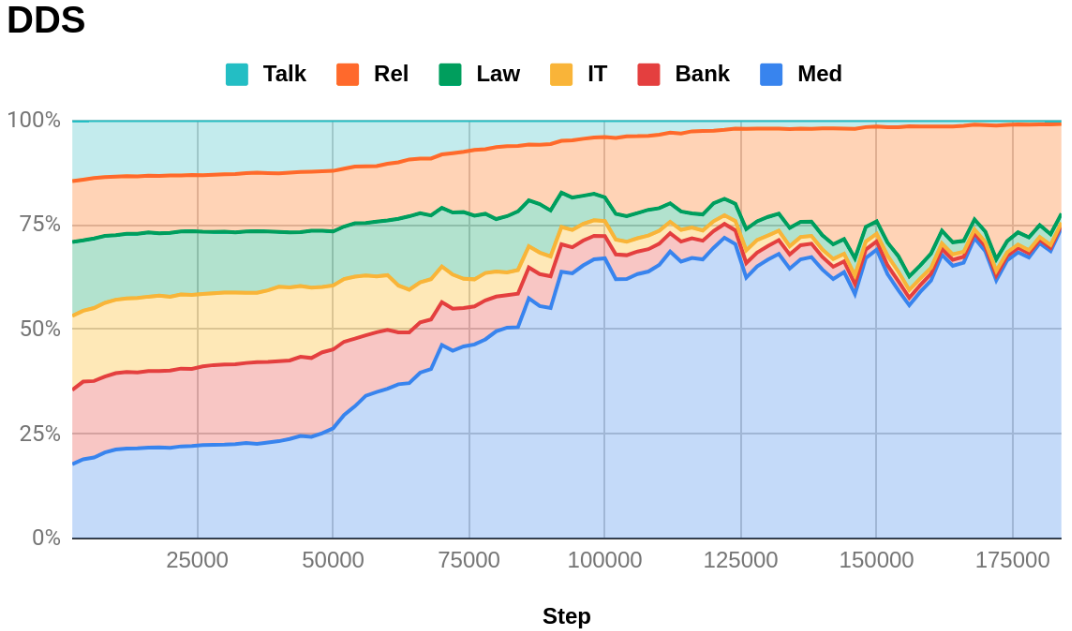
\includegraphics[width=0.97\textwidth]{DDS.png}  
  \caption{DDS}
  \label{fig:DDS}
\end{subfigure}
\begin{subfigure}{.5\textwidth}
  \centering
  % include second image
  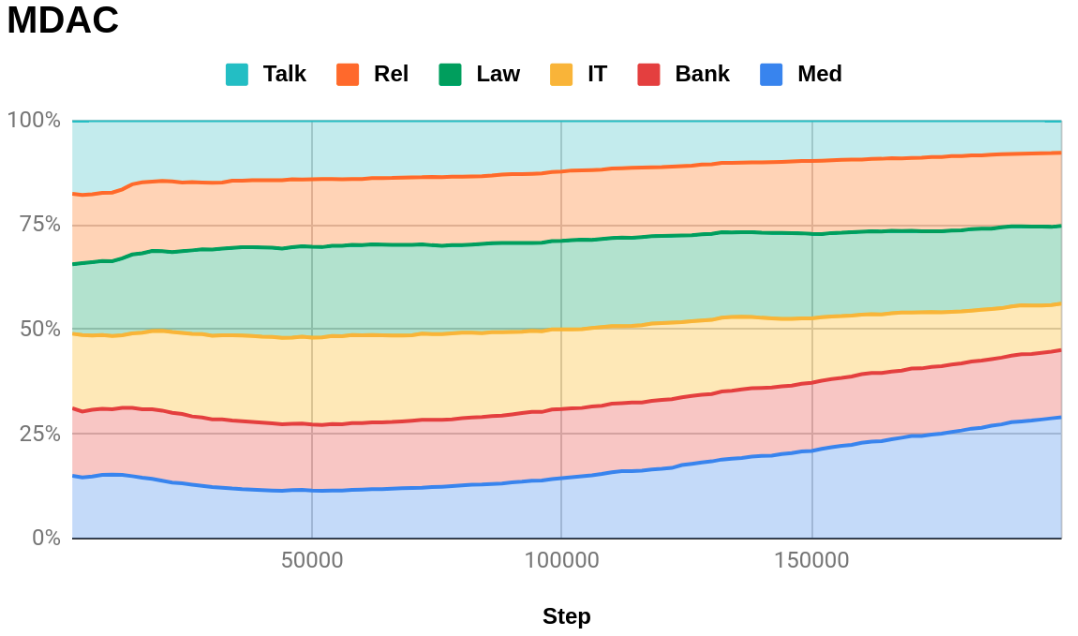
\includegraphics[width=0.97\textwidth]{MDAC.png}  
  \caption{MDAC}
  \label{fig:MDAC}
\end{subfigure}
\caption{Evolution of the sampling distribution during training.}
\label{fig:sampling}
\end{figure*}

\begin{table*}[htbp]
  \vspace{-2\baselineskip}
  \centering \small
  \begin{tabular}{|l|*{10}{r|}} \cline{1-2} \cline{4-11}
    domain \hfill $d=$ & \multicolumn{1}{c|}{\domain{news}}& \hfill &domain \hfill $d=$ & \multicolumn{1}{c|}{\domain{ med}} & \multicolumn{1}{c|}{\domain{ law}} & \multicolumn{1}{c|}{\domain{bank}} & \multicolumn{1}{c|}{\domain{talk}} & \multicolumn{1}{c|}{\domain{ it }} & \multicolumn{1}{c|}{\domain{ rel}} & \multicolumn{1}{c|}{mean}  \\ 
\cline{1-2} \cline{4-11}
    \multicolumn{2}{|c|}{\sl Unseen domain} & &\multicolumn{8}{c|}{\sl Training with 30 clusters} \\ 
\cline{1-2} \cline{4-11}
    \system{Mixed-0}      & 25.7 & &\system{DDS($\vlambda^*, \vlambda_d$)}&38.3&60.1&50.3&35.8&49.1&90.1&53.9\\
    \system{Mixed-0.25} & 25.8 & &\system{MDAC($\vlambda^*, \vlambda_d$)}&39.2$^*$&61.6$^*$&52.0$^*$&38.2$^*$&49.1&89.7&55.0$^*$\\ \cline{4-11}
    \system{Mixed-0.5}   &26.5\\
    \system{Mixed-0.75} &26.8\\
    \system{Mixed-1} &26.9 \\
    \cline{1-2}
     \system{DDS($\vlambda_0, \vlambda_{news}$)} &26.3 \\
     \system{MDAC($\vlambda_0, \vlambda_{news}$)} &26.3 \\
     \cline{1-2}
  \end{tabular}
  \caption{Unseen domain adaptation (left) and automatic clustering adaptation (right). For a given line, each column corresponds to one distinct system. ($^*$) MDAC is significantly better than DDS.}
  \label{tab:unsupervised-da}
\end{table*}

\subsection{Unseen domain}\label{ssec:uda}
The left part of Table~\ref{tab:unsupervised-da} displays the performance on the unseen domain \domain{news} for systems trained with mixtures $\vlambda^l \in \big[ \vlambda_0, \vlambda_{0.25}, \vlambda_{0.5}, \vlambda_{0.75}, \vlambda_{1.0}\big]$ and with dynamic data selection (MDAC and DDS). These systems have insignificant differences in BLEU, suggesting that dynamic mixtures do not improve the robustness of NMT systems against unseen domains. However, the performance of MDAC and DDS remains close to the best performance, showing that they also apply in such settings. % the robustness of the NMT model.

\subsection{Automatic clustering}\label{ssec:clda}
The right part of Table~\ref{tab:unsupervised-da} reports the performance of NMT systems adapted to each domain.
% \footnote{A more detailed analysis is in the supplementary material.}
In comparison to Section~\ref{ssec:da}, the training data is distributed in 30 automatic clusters instead of the 6 original domains. Splitting the train data into small groups gives the learner extra degrees of freedom when selecting the best distribution. However, as these clusters are built automatically, they are noisier in nature. According to results in Table~\ref{tab:unsupervised-da}, this scenario is hard both for DDS and MDAC, which performs much worse than for the supervised DA setting. This again signals the importance of initialization: analyzing the clustering, we find that the data for \domain{rel} mostly correspond to one single cluster. With a uniform initialization, this cluster starts with a small weight and never succeeds in matching the good performance observed in the DA setting.

\section{Related Work \label{sec:related}}

Domain adaptation is an old problem that has been studied from many angles, both for SMT and NMT. A survey of supervised and unsupervised DA for NMT is in \cite{Chu2017comparison}, where the authors distinguish between data-centric and model-centric DA, a view also adopted in the recent survey of \newcite{Saunders21asurvey}. Our approach to DA in this paper falls under the former category. We refer readers interested in DA to these papers.

Multidomain NMT (MDMT) aims to develop systems that simultaneously bode well for several domains. Like for DA, techniques for supervised MDMT combine one or several ingredients: (a) the specialization of data representations \cite{Kobus17domaincontrol} or of sub-networks \cite{Pham19generic} to differentiate the processing of each domain; (b) the use of adversarial techniques to neutralize differences between domains \cite{Britz17mixing,Zeng18multidomain}; (c) the use of automatic domain identification e.g.\ \cite{Jiang19multidomain}. Unsupervised MDMT is studied in \cite{Farajian17multidomain}, as an instance of unsupervised DA.

Most approaches to adaptive/dynamic data selection take inspiration from \newcite{Bengio09curriculum}, where the notion of curriculum learning is introduced. CL relies on the notion of the ``easiness'' of a sample to schedule the presentation of training data so as to start with the easiest examples and end with the hardest. Various ways to automate CL in the framework of multi-armed bandits are explored in \cite{Graves17automated}, which has been an inspiration for our implementation. While the initial aim was primarily to improve and speed up training, CL has also proven useful for multidomain and multilingual MT, based on alternative definitions of ``easiness''.\fyDone{Ajouter Grave}
For instance, \newcite{Zhang19curriculum} study supervised DA and propose a curriculum approach which progressively augments the training data: early stages only use in-data, while less relevant\footnote{Domain distance is computed with Lewis-Moore scores (based on the cross-entropy of in-domain LM).} data are introduced in later stages. This is opposite to the policy of \newcite{Vanderwees17dynamic}, whose \emph{gradual fine-tuning} progressively increases the focus on in-domain data.\fyDone{These have not been compared? and also to what we do ?} 

\newcite{Kumar19reinforcement} use reinforcement learning to learn the curriculum strategy: in this work, complexity corresponds to difficulty levels which are binned using contrastive data selection. The reward is based on the increase of the devset loss that results from the current data selection strategy.\fyDone{Alert: what do we do during warm-up ?} This technique is applied to multilingual NMT in \cite{Kumar21learning}. \newcite{Zhou20uncertainty} propose another CL-based approach which relies on \emph{instance uncertainty} as a measure of their difficulty and presents data samples starting with the easiest. Another contribution of this work is a new stopping criterium. Closest to our problems, \newcite{Wang20learning-multi} adapt CL for multidomain NMT, where an optimal instance weighting scheme is found using Bayesian optimization techniques. Each step consists of (a) weighting instances based on relevance features, (b) fine-tuning a pretrained model using the weighted training set, and is applied to train a sequence of models. The one that maximizes the devset performance is finally retained.

\section{Conclusion and outlook \label{sec:conclusion}}
\fyDone{Write conclusion}
In this study, we have presented a generic framework to perform multiple adaptation tasks for machine translation, ranging from supervised domain adaptation to multidomain NMT and unseen domain adaptation. In our experiments, we have shown that the same algorithm, aimed at automatically finding an effective data sampling scheme during the course of training, can be used in all these situations. This algorithm, we believe, provides us with a more sound approach to (multi-domain) DA than existing heuristics and dispenses with the costly search of optimal meta-parameters. Another contribution of our work is an experimental comparison of recent approaches to dynamic data selection.

Our future work will continue developing this approach and improve its effectiveness. One issue that we have left unaddressed is reward normalization, which is especially important in the early stages of training \cite{Kumar19reinforcement}. Another area where we need to progress is the unsupervised learning setting of \textsection~\ref{ssec:clda}, where our results lag behind supervised DA. This might be due to the inability of our simplistic optimization strategy to handle situations where the number of clusters is large.
%\clearpage{}
% slow down learning during warm up or normalize reward; handle large number of classes;
% too much importance to the dev ? randomize ?

\bibliography{multidomain}
\bibliographystyle{eamt22}

% \clearpage{}

% \appendix
%\section*{A - Generalized Multi-Domain Dynamic Adaptation Curriculum Algorithm}
The pseudo-code for the generalized Multi-Domain Adaptation Dynamic Sampling Algorithm  is in algorithm~\ref{alg:mdmt}.
\begin{breakablealgorithm}
\caption{Multi-Domain Adaptation Dynamic Sampling} \label{alg:mdmt}
\begin{algorithmic}[1]
\REQUIRE {
  \begin{itemize}
    \setlength{\itemsep}{-1pt}    \setlength{\parsep}{0pt}
  \item[] 
  \item $n_d$ corpora $C^d, d \in [1, \dots,n_d]$ for $n_d$ domains equipped by an empirical distribution $D_d(x)$
  \item $n_d$  dev sets $Dev^d, d\in [1, \dots,n_d]$ for $n_d$ domains.
  \item Domain testing distribution $\vlambda^t \in \mathbb{R}^{n_d}$
  \item Batch size $B$
  \item Domain Dynamic Sampling Distribution $\lambda^l_i \in \mathbb{R}^{n_d}$ where $i$ indexes iterations.
  \item $Eval\_scores = []$
  \item $Early\_stopping$ criterion
  \item Total training iterations $iter\_num$
  \item Update rule for sampling distribution $\vlambda^l_i$
 \end{itemize}}
\REPEAT 
\STATE{// Start of iteration i}
\STATE{Randomly pick $d \in [1,\dots,n_d]$ from sampling distribution $\lambda^l_i$}
\STATE{Sample $B$ sentences from $C^d$ with empirical distribution $D_d(x)$}
\STATE{Update model by applying SGD computed from $B$ sampled sentences}
\IF{$i \equiv 0 \mod{eval\_step}$}
	\STATE{Evaluate current model with $n_d$ dev sets. $S^d_i$ is the performance at iteration $i^{th}$ on domain $d$}
	\STATE{Report weighted score using test distribution $\vlambda^t$. $$eval(i) = \displaystyle{\mathop{\sum}_d^{n_d} \lambda^t(d) S^d_i}$$}
	\STATE{$Eval\_scores.append(eval(i))$}
\ENDIF
\IF{$i \equiv 0 \mod{sampler\_updating\_step}$}
	\STATE Update $\vlambda^l_i$
\ENDIF
\IF{$Early\_stopping(Eval\_scores)$}
	\STATE{break}
\ENDIF
\STATE{$i=i+1$}
\UNTIL{$i> iter\_num$}
\end{algorithmic}
\end{breakablealgorithm}
\section*{B - Experiments with automatic domains}
\begin{table*}[htbp]
  \centering
  \footnotesize
  \begin{tabular}{|p{0.5cm}|*{7}{c|}|*{6}{c|}} 
  \hline
\multirow{2}*{Cl. }&\multirow{2}*{size}&\multicolumn{6}{c||}{Domain content}&\multicolumn{6}{c|}{MDAC systems}\\
  \cline{3-14}
&&MED&ECB&IT&LAW&REL&TALK&MED&ECB&IT&LAW&REL&TALK \\
\hline
1&27436&0.24&0.11&0.47&0.17&0.00&0.01&0.01&0.00&0.01&0.00&0.00&0.01 \\
2&68108&0.48&0.04&0.19&0.28&0.00&0.00&0.02&0.03&0.02&0.01&0.02&0.02 \\
3&182594&1.00&0.00&0.00&0.00&0.00&0.00&0.03&0.06&0.04&0.06&0.03&0.03 \\
4&323474&0.05&0.06&0.01&0.87&0.00&0.00&0.03&\underline{0.07}&0.03&\underline{0.20}&0.03&0.04 \\
5&137451&0.03&0.00&0.00&0.00&0.86&0.10&0.03&0.04&0.04&0.06&\underline{0.17}&0.04 \\
6&109949&0.44&0.04&0.40&0.07&0.01&0.04&0.04&0.06&0.04&0.05&0.02&0.03 \\
7&133395&0.92&0.01&0.01&0.05&0.00&0.00&0.03&0.04&0.03&0.05&0.05&0.03 \\
8&91464&0.98&0.00&0.00&0.02&0.00&0.00&0.04&0.03&0.04&0.04&0.05&0.03 \\
9&61353&0.02&0.01&0.96&0.01&0.00&0.00&0.03&0.02&0.03&0.01&0.04&0.02 \\
10&301639&0.98&0.00&0.00&0.02&0.00&0.00&0.02&0.01&0.01&0.01&0.02&0.03 \\
11&225347&0.93&0.00&0.01&0.04&0.00&0.01&0.03&0.04&0.04&0.02&0.03&0.04 \\
12&92982&0.98&0.00&0.01&0.01&0.00&0.00&0.04&0.02&0.03&0.01&0.03&0.03 \\
13&356377&0.99&0.00&0.00&0.01&0.00&0.00&0.03&0.03&0.04&0.03&0.03&0.04 \\
14&17260&0.03&0.37&0.01&0.59&0.00&0.00&0.03&0.03&0.03&0.02&0.03&0.02 \\
15&333957&0.98&0.00&0.01&0.01&0.00&0.00&0.04&0.02&0.03&0.01&0.03&0.03 \\
16&136944&0.02&0.89&0.01&0.08&0.00&0.00&0.04&\underline{0.08}&0.03&0.04&0.03&0.04 \\
17&30443&0.96&0.01&0.02&0.01&0.00&0.00&0.04&0.03&0.03&0.03&0.04&0.03 \\
18&54378&0.93&0.00&0.05&0.02&0.00&0.00&0.04&0.04&0.02&0.03&0.07&0.03 \\
19&245000&0.99&0.00&0.00&0.00&0.00&0.00&0.04&0.04&0.03&0.03&0.04&0.03 \\
20&27227&0.15&0.00&0.79&0.05&0.00&0.01&0.04&0.03&0.03&0.02&0.04&0.03 \\
21&182990&0.99&0.00&0.00&0.01&0.00&0.00&0.03&0.02&0.03&0.03&0.03&0.03 \\
22&222802&0.21&0.01&0.40&0.04&0.02&0.32&0.04&0.04&\underline{0.08}&0.02&0.01&\underline{0.08} \\
23&27534&0.11&0.48&0.02&0.39&0.00&0.00&0.03&0.03&0.05&0.02&0.01&0.04 \\
24&47065&0.99&0.00&0.01&0.00&0.00&0.00&0.04&0.02&0.05&0.05&0.03&0.04 \\
25&8129&0.95&0.00&0.04&0.01&0.00&0.00&0.03&0.03&0.04&0.03&0.02&0.02 \\
26&28237&0.59&0.02&0.23&0.11&0.00&0.05&0.03&0.02&0.02&0.01&0.03&0.02 \\
27&134828&0.53&0.00&0.02&0.00&0.01&0.44&0.04&0.03&0.03&0.01&0.01&0.05 \\
28&109324&0.99&0.00&0.00&0.01&0.00&0.00&0.04&0.03&0.03&0.02&0.01&0.02 \\
29&25561&0.56&0.16&0.08&0.16&0.00&0.04&0.03&0.03&0.03&0.02&0.02&0.03 \\
30&109260&0.01&0.06&0.00&0.92&0.00&0.00&0.03&0.03&0.03&0.06&0.04&0.04 \\
\hline
\end{tabular}
\caption{Automatic clustering experiments. We report the size of each cluster. In the 6 left columns, each line gives the proportions of the domains in each cluster. In the 6 right columns, each column corresponds to a MDAC experiment; each line gives the cumulated proportion of the corresponding cluster in the training data. For instance, when targeting the domain \domain{ecb}, cluster~4 (mostly \domain{law}) is sampled with a probability of $0.07$, and cluster~16 (mostly \domain{ecb}) is sampled with probability $0.08$. For each system, we underline the most often sampled clusters.}
\label{tab:automatic_domains}
\end{table*}

This experiment aims to simulate with automatic domains a scenario where the number of ``domains'' is large and where some ``domains'' are close and can effectively share information. Full results are in Table~\ref{tab:automatic_domains}. Cluster sizes vary from approximately 8k sentences (cluster~24) up to more than 350k sentences. More than 2/3 of these clusters mostly comprise texts from one single domain, as for cluster 12, which is predominantly \domain{med}, the remaining clusters typically mix 2 domains. According to the table, for each system, the clusters most sampled by MDAC contain most of the data of the corresponding domain. This demonstrates that MDAC is able to find related data to the task automatically. However, MDAC performance is still far behind that of the supervised scenario, as we explain in the paper. 
\\
\\
\\
%%%%%%%%%%%%%%%%%%%%%%%%%%%%%%%%


\end{document}